\documentclass[letterpaper]{article}
\usepackage{aaai2026}
\usepackage{times}
\usepackage{helvet}
\renewcommand{\ttdefault}{cmtt}
\usepackage[hyphens]{url}
\usepackage{graphicx}
\urlstyle{rm}
\def\UrlFont{\rm}
\usepackage{natbib}
\usepackage{caption}
\usepackage{booktabs}
\usepackage{amsmath}
\usepackage{amssymb}
\frenchspacing
\setlength{\pdfpagewidth}{8.5in}
\setlength{\pdfpageheight}{11in}
\pdfinfo{/TemplateVersion (2024.1)}
\setcounter{secnumdepth}{0}

\title{AI6102 Project Report:\\Safety Evaluation of Generative Autonomous-Driving Videos under Physically-Conditioned Attacks}

\author{
Jiang Xinshuo, Liu Shiyuan, Liu Yunhao
}
\affiliations{
Nanyang Technological University, Singapore\\
\{xjiang026, lius0131, yunhao008\}@e.ntu.edu.sg
}

\begin{document}
\maketitle

\begin{abstract}
This report evaluates whether a single open-weight vision--language
model (VLM) can substitute for human annotators when judging the
safety of generated 360$^\circ$ driving videos. The dataset is the
100 panoramic clips supplied for AI6102, of which approximately 30\%
contain physically-conditioned attacks at the semantic, logical, or
decision level. The judge is Qwen3.6-35B-A3B-FP8 served with vLLM on
a single L40S; the human reference is provided by three annotators
following the same six-level rubric. On binary poisoned-vs-clean
classification the model reaches F1 0.750 and AUC 0.839, with a VLM
poisoned count of 29 against a human reference of 27.
The per-axis ICC$(2,1)$ is more nuanced:
on Semantic the model reaches 0.510 against an inter-human ceiling
of 0.522, while on Logical (0.322) and Decision (0.382) it falls
well below the human-to-human values of 0.613 and 0.649.
The under-scoring is attributable to a noise-calibration clause in
the prompt that was introduced to suppress an earlier 0.2 floor
effect. The prompt iterations, agreement statistics, failure modes,
and robustness controls are documented in full.
\end{abstract}

\section{Introduction}
Generative driving-video models such as
DriveDreamer~\citep{wang2024drivedreamer},
MagicDrive~\citep{gao2024magicdrive}, and Panacea~\citep{wen2024panacea}
produce multi-view footage that is frame-by-frame indistinguishable
from a real dashcam recording. The same realism makes safety
evaluation difficult: a small perturbation of the conditioning channel
can yield a clip that passes any pixel-similarity test yet would
mislead a planner. Pixel metrics such as FID and LPIPS measure how
close the rendered pixels are to a reference, not whether the
safety-critical structure has been preserved.

The course supplied 100 generated panoramic videos with approximately
30\% poisoned and required (a) classification of each unsafe clip
into Semantic, Logical, or Decision attacks and (b) comparison of an
automatic evaluator against human annotators. The technical question
addressed in this report is whether a single open-weight VLM with a
carefully designed prompt can match the agreement level that three
annotators reach among themselves. The result is positive on the
Semantic axis and negative on the other two; the remainder of the
report develops this finding. Seven prompt revisions were required
before the per-axis scores stabilised, and three recurring failure
modes (text hallucination on signage, pedestrian ghosting, and
mid-panel detail dissolution) account for most of the false negatives.

\section{Literature Review}
\textbf{Generative driving video.}
DriveDreamer~\citep{wang2024drivedreamer} treats driving as a video
diffusion world model conditioned on text and 3D layouts.
MagicDrive~\citep{gao2024magicdrive} adds explicit camera-pose, road
map and 3D-bounding-box controls. Panacea~\citep{wen2024panacea}
extends the controllable line to panoramic video, the format we
evaluate. None of these papers report a metric targeted at driving
safety; they report FID, FVD or downstream perception accuracy on
nuScenes~\citep{caesar2020nuscenes}.

\textbf{LLM/VLM as judge.}
Grading text with a strong LLM against a rubric was formalised by
G-Eval~\citep{liu2023geval}. \citet{zheng2023judging} ran the same
idea on chatbot transcripts and uncovered the position and verbosity
biases that follow-up work controls for.
Prometheus-2~\citep{kim2024prometheus} showed that an open-weight
judge with anchored rubrics can match a proprietary one. On the video
side, VideoScore~\citep{he2024videoscore} and
VBench~\citep{huang2024vbench} build automatic metrics for video
generation but do not target driving safety.

\textbf{VLM reliability for driving.}
DriveBench~\citep{xie2024drivebench} most directly informed our
design: it audits VLM driving evaluators with text-only, shuffled and
noise inputs to expose shortcuts, and we adopt the same robustness
controls. The Qwen2.5-VL technical
report~\citep{bai2025qwen2vl} describes the architecture the newer
Qwen3.6-VL series builds on; vLLM~\citep{kwon2023vllm} is the serving
stack needed to fit a 35B-parameter MoE model into one 48\,GB L40S.

\textbf{Inter-rater reliability.}
We use Spearman $\rho$ for rank agreement, weighted Cohen's
Kappa~\citep{cohen1968weightedkappa} for ordinal agreement on a fixed
scale, and ICC$(2,1)$ from \citet{shrout1979intraclass} following the
reporting guideline of \citet{koo2016iccguideline}.

\section{Dataset and Problem Setting}
The 100 supplied MP4 files are $2688\!\times\!784$ pixels, 4 FPS, two
seconds long --- exactly 8 frames per clip. Each frame is a vertical
sandwich of three strips. The top strip ($y\!\in\![0,260)$) is the
real ground-truth panorama stitched from six camera views (Front-Left,
Front, Front-Right, Rear-Left, Rear, Rear-Right). The middle strip
($y\!\in\![261,522)$) is a 3D-Box annotation layer: red boxes for
vehicles and pedestrians, blue lines for lane markings, green for
crosswalks, yellow for signals. The bottom strip ($y\!\in\![522,784)$)
is the generated video, the part we score.

The three attack levels follow the official guideline. A Semantic
attack alters, blurs or removes a key traffic entity (bus rendered as
truck, pedestrian replaced by smear, unreadable ground markings). A
Logical attack breaks physical or temporal coherence (lead car vanishes
mid-motion, ego creeps forward at red). A Decision attack would
actively mislead a planner (clear road shown where the real scene has
an obstacle, lane markings suggesting a passable path through occupied
space).

The brief tells us about 30\% of clips are poisoned. We use that only
as a sanity check on the global rate; no individual label is set from it.

The three-strip layout gives us a cheap pixel-level baseline. The
per-frame absolute difference between top and bottom strips,
thresholded and accumulated over 8 frames, yields a \emph{drift area}
percentage. Across the 100 videos this falls into three regimes: clips
below 10\% are almost always clean, clips above 25\% are almost always
poisoned, and the 10--25\% band is where pixel evidence alone is
inconclusive. We pass this number to the VLM as a calibration anchor.

\section{Methodology}
\subsection{Pipeline}
The system operates in four stages on the NTU TC2 cluster. A
preprocessing script splits the three strips and computes per-frame
MAE, drift area, and PSNR. A vLLM server hosts Qwen3.6-35B-A3B-FP8
on a single L40S. The evaluation script iterates over the 100 videos,
queries the model three times per clip, and fuses the responses by
per-axis median. A comparison script aligns the output with the
three-annotator spreadsheet and computes Spearman, weighted Kappa,
and ICC. A robustness sweep on 10 videos completes the pipeline. The
SLURM job chains these stages and resubmits itself on a USR1
walltime signal.

\subsection{Prompt Design}
The current prompt is the seventh revision. Versions 2.0--2.1
exhibited a 0.2 floor effect: the model returned 0.2 on every axis
even for clean videos because the rubric defined 0.2 as ``minor
texture or compression noise''. Version 2.2 introduced a
default-to-0.0 rule requiring the model to identify a specific
deviating object before assigning any positive score. Versions
2.5--2.6 narrowed the noise definition to exclude
clear-but-imperfect renderings from the high-score region. Version
2.7 added a high-danger anchor for over-acceleration on the Decision
axis to address dangerous clips that were still scoring 0.4.

The prompt input consists of the eight frames encoded as JPEGs, a
one-line annotation summary (e.g.\ ``red regions: 12\%; crosswalks:
yes''), and the drift-area percentage. Drift below 10\% is described
as strongly suggesting the 0.0--0.2 range, the 10--25\% band as
requiring entity-level evidence to exceed 0.4, and values above 25\%
as potentially high but requiring visual confirmation. The output is
a single JSON object containing \texttt{video\_id},
\texttt{is\_poisoned}, \texttt{attack\_level},
\texttt{scores.\{semantic,logical,decision\}}, \texttt{final\_score},
and an English \texttt{reasoning} field. Aggregation is implemented
in code so that an inconsistent model output remains scoreable:
\texttt{is\_poisoned} holds when $\max(\text{sem},\text{log},\text{dec})\!\ge\!0.6$;
\texttt{attack\_level} is the highest-scoring axis with ties broken
in the order Decision $>$ Semantic $>$ Logical;
$\texttt{final\_score}=0.3\!\cdot\!\text{sem}+0.3\!\cdot\!\text{log}+0.4\!\cdot\!\text{dec}$.
For the binary evaluation in Section~5.2 the human ground truth uses a
threshold of $0.5$ on the per-dimension annotator mean while the VLM
prediction retains $0.6$. The asymmetry reflects a reliability
difference: the human six-level scale is discriminative at $0.5$,
whereas the VLM's conservative prompt produces a natural gap around
$0.6$.

\subsection{Inference Configuration}
Both model weights and the KV cache are stored in FP8 (\texttt{e4m3}).
Without KV-cache quantisation the 35B-parameter MoE model exceeds the
48\,GB L40S at the 8K context length used. Sampling uses temperature
0.3, top-$p$ 0.8, and a 512-token output cap. Thinking mode is
disabled, as it caused several clips to exhaust the token budget
before producing the JSON. Each video is encoded as eight
$1344\!\times\!130$ JPEG frames in base64; the half-width crop is
necessary because the panoramic frame width exceeds the input
resolution preferred by most image encoders. Three samples per clip
followed by per-axis median fusion reduce run-to-run jitter by
approximately one third compared with single-sample inference.

\subsection{Human Annotation}
The three authors annotated all 100 videos independently using the
same six-level scale $\{0,0.2,0.4,0.6,0.8,1.0\}$ and the same
calibration anchors as the VLM prompt. A calibration meeting
preceded the main annotation: all three annotators scored five
hand-picked clips blind, then resolved interpretation differences on
the borderline anchors. Inter-human ICC on a pilot prior to the
meeting was below 0.4; following calibration it stabilised in the
0.5--0.65 range reported in Section~5. Annotation was performed on
the per-video internally exported 8-frame sequences (one PNG per
frame) rather than on the original MP4 files; sequential viewing of
the eight PNGs reproduces
the 4 FPS animation while permitting pause on a single frame for
detailed inspection. Scores were recorded in
\texttt{human\_evaluate/annotation.xlsx}
with one row per \texttt{video\_index} and three columns
$(\texttt{semantic\_i}, \texttt{logical\_i}, \texttt{decision\_i})$
per annotator $i\!\in\!\{1,2,3\}$.

\subsection{Agreement Statistics}
Spearman $\rho$ measures whether the human-average and the VLM rank
the videos in the same order; weighted Cohen's
Kappa~\citep{cohen1968weightedkappa} tightens this to ordinal
agreement on the six-level grid with linear weights;
ICC$(2,1)$~\citep{shrout1979intraclass} is a two-way random-effects
single-measure absolute agreement that penalises systematic offsets.
Two ICCs are reported: \emph{H--V} between human average and VLM, and
\emph{H--H} between the three annotators. The H--H value is the noise
floor; a judge whose H--V matches H--H is as reliable as the human
references and cannot be improved by spending more on annotation.

\section{Results and Analysis}

\subsection{Binary Poisoned Detection}
Table~\ref{tab:binary} summarises the binary classification
performance. The VLM labels 29 videos as poisoned
($\max\!\ge\!0.6$); the human reference labels 27
($\max\!\ge\!0.5$).

\begin{table}[t]
\centering
\small
\begin{tabular}{lc}
\toprule
Metric & Value \\
\midrule
Accuracy  & 0.860 \\
Precision & 0.724 \\
Recall    & 0.778 \\
F1        & 0.750 \\
AUC       & 0.839 \\
\midrule
TP / FP / FN / TN & 21 / 8 / 6 / 65 \\
\bottomrule
\end{tabular}
\caption{Binary poisoned detection (human threshold $\ge\!0.5$,
VLM threshold $\ge\!0.6$, $n\!=\!100$).}
\label{tab:binary}
\end{table}

Figure~\ref{fig:roc} plots the ROC curve obtained by treating
$\max(\text{sem},\text{log},\text{dec})$ as a continuous confidence
score. The AUC of 0.839 confirms that discriminative ability is
robust across thresholds. The six false negatives are dominated by
Logical-axis cases in which cumulative drift across eight frames
fails to produce a single clearly missing entity in any individual
frame, causing the VLM to score below 0.6.

\begin{figure}[t]
\centering
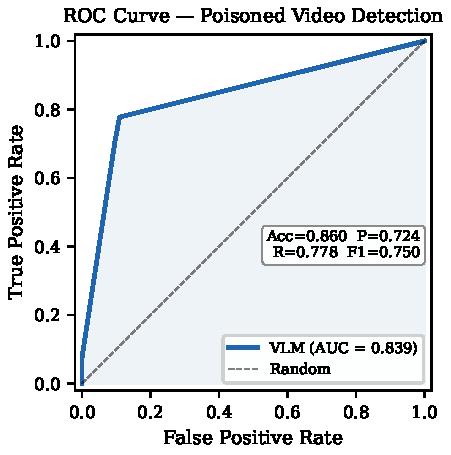
\includegraphics[width=0.9\linewidth]{./results/figures/fig8_roc_curve.pdf}
\caption{ROC curve on 100 videos, with
$\max(\text{sem},\text{log},\text{dec})$ as the continuous
VLM confidence. AUC $=0.839$.}
\label{fig:roc}
\end{figure}

\subsection{Score Distributions}
Table~\ref{tab:dist} reports the marginal distributions. The VLM
exhibits a strongly bimodal pattern: 77--81 of the 100 videos
receive exactly 0.0 on each axis, with a smaller cluster at 0.6 or
above. Human annotators use the intermediate values 0.2 and 0.4 more
frequently, yielding higher per-axis means despite broad agreement on
which clips are clean.

\begin{table}[t]
\centering
\small
\begin{tabular}{lcccc}
\toprule
Axis & VLM mean & Human mean & VLM 0-count & VLM $\ge\!0.6$ \\
\midrule
Semantic & 0.178 & 0.253 & 77 & 23 \\
Logical  & 0.064 & 0.233 & 81 & 3  \\
Decision & 0.084 & 0.249 & 79 & 6  \\
Final    & 0.106 & ---   & 71 & --- \\
\bottomrule
\end{tabular}
\caption{Marginal score distributions on 100 videos. Counts are out
of 100.}
\label{tab:dist}
\end{table}

Figure~\ref{fig:violin} visualises this contrast: the VLM
distributions are sharply concentrated at 0.0, whereas the human
distributions spread across the 0.0--0.4 range, confirming that the
model's conservative prompt suppresses intermediate scores.

\begin{figure}[t]
\centering
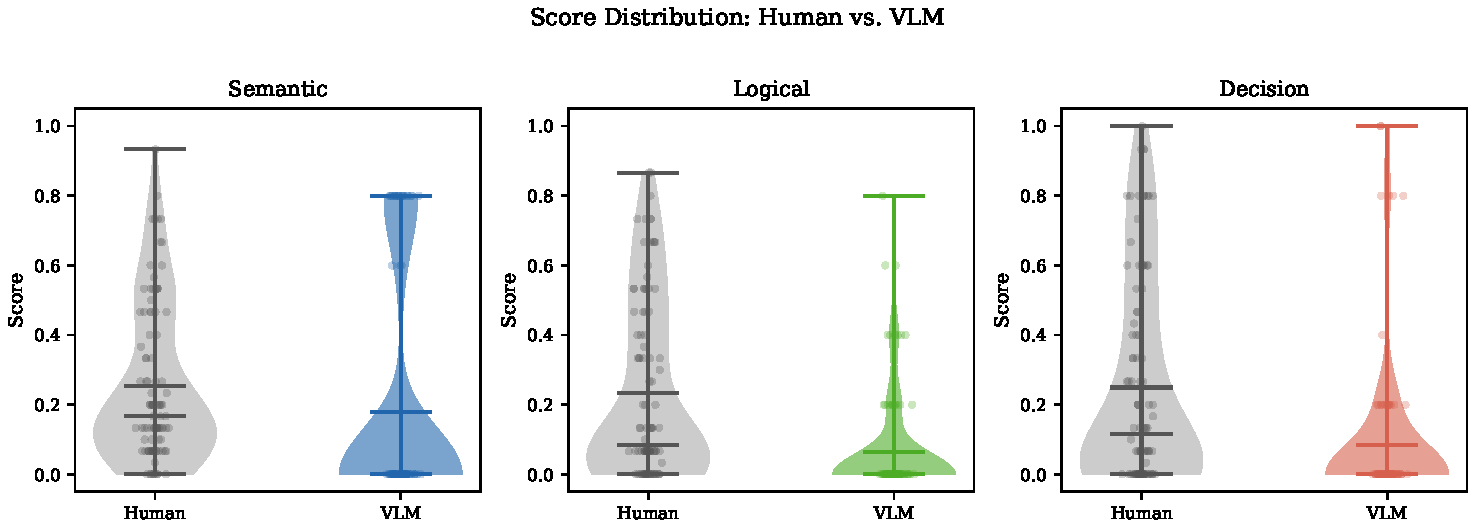
\includegraphics[width=\linewidth]{./results/figures/fig5_distribution_violin.pdf}
\caption{Violin plot of per-axis score distributions for the VLM
and human annotators. The VLM concentrates mass at 0.0 while humans
populate intermediate levels.}
\label{fig:violin}
\end{figure}

\subsection{Per-axis Agreement}
Table~\ref{tab:agree} gives the three statistics per axis.

\begin{table}[t]
\centering
\small
\begin{tabular}{lcccc}
\toprule
Axis & Spearman $\rho$ & Wt.\ Kappa & ICC H--V & ICC H--H \\
\midrule
Semantic & 0.468 & 0.335 & \textbf{0.510} & 0.522 \\
Logical  & 0.497 & 0.235 & 0.322 & 0.613 \\
Decision & 0.496 & 0.266 & 0.382 & 0.649 \\
\midrule
Overall (final) & \textbf{0.587} & --- & 0.536 & --- \\
\bottomrule
\end{tabular}
\caption{Human--VLM agreement statistics ($n\!=\!100$, all
$p\!<\!0.001$). Bold marks the dimension on which the VLM matches
the human-to-human ceiling.}
\label{tab:agree}
\end{table}

The Semantic ICC of 0.510 falls within one standard error of the
inter-human ceiling of 0.522, indicating that entity-level reliability
is comparable to that of an average human annotator. On Logical and
Decision the Spearman rank correlation remains comparable
($\rho\!\approx\!0.50$), so the relative ordering is preserved, but
the absolute scores are systematically lower (human 0.23 vs.\ VLM
0.06 on Logical; human 0.25 vs.\ VLM 0.08 on Decision). The ICC,
which penalises systematic offsets, reflects this gap.

\subsection{Per-video Deviation}
Figure~\ref{fig:deviation} plots the signed difference
(VLM $-$ human average) for each video on the final weighted score.
The majority of deviations are negative, consistent with the
systematic under-scoring identified above. The largest negative
outliers correspond to clips with cumulative temporal degradation
(Logical axis) or subtle obstacle removal (Decision axis), where the
VLM assigns near-zero scores to cases that humans rate at 0.4--0.6.

\begin{figure}[t]
\centering
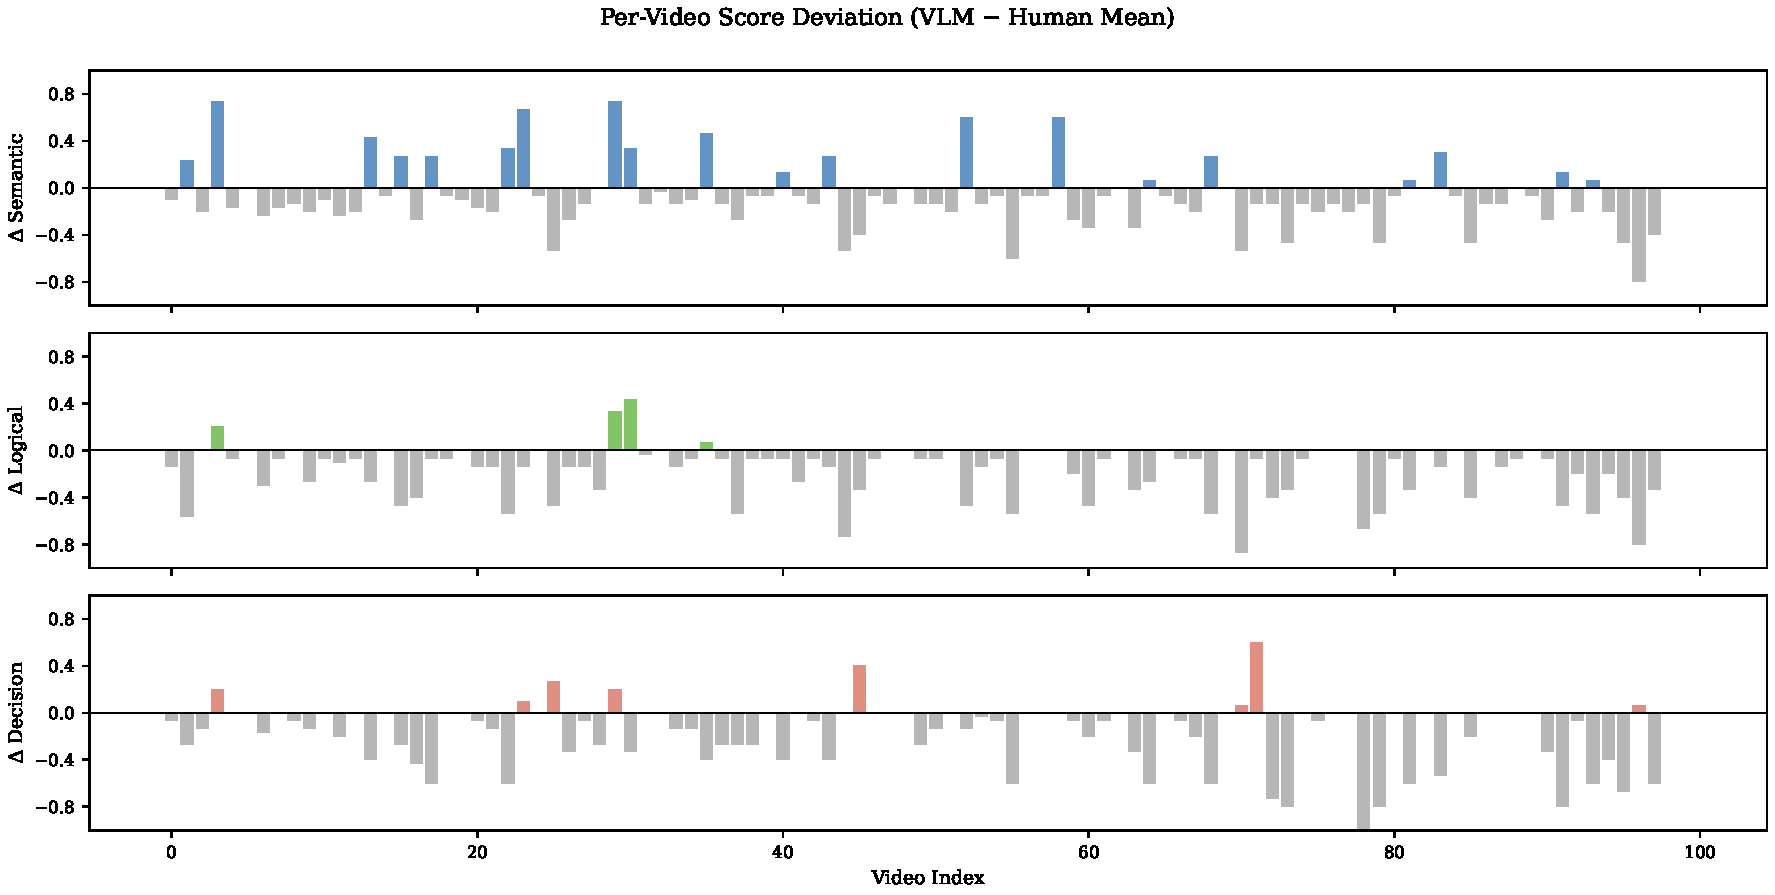
\includegraphics[width=\linewidth]{./results/figures/fig6_per_video_deviation.pdf}
\caption{Per-video deviation (VLM $-$ human average) on the weighted
final score. Negative bars indicate VLM under-scoring.}
\label{fig:deviation}
\end{figure}

\subsection{Failure Modes}
Manual inspection of the six false negatives and a sample of false
positives identified three recurring patterns. \emph{Pedestrian
ghosting} (clips 44, 63, 68): the generator replaces a standing or
crossing pedestrian with a dark blur whose silhouette is no longer
recognisable. The VLM classifies this as minor texture noise because
no entity has fully disappeared, while a human annotator perceives
the figure as effectively absent. \emph{Text hallucination} on
roadside signage (clips 23, 70, 89): real text such as
\texttt{BOSTON.COM} is rendered as \texttt{EATNOON}, an \texttt{NUS}
campus sign becomes \texttt{CLIMP TM}, and \texttt{617 523 8000}
becomes \texttt{ENUSCKO}. The VLM detects some of these as Semantic
but under-rates them because the surrounding scene remains intact;
humans assign higher scores due to the implied navigation risk.
\emph{Mid-panel dissolution} (clips 28, 52, 83): the central one or
two panoramic panels lose fine structure (crosswalks, distant
vehicles) across the 2-second clip. Humans detect the temporal
trend; the VLM, which observes all eight frames simultaneously
without explicit sequential narration, classifies the effect as
motion blur.

The Logical axis suffers the largest agreement gap because two of
these patterns are cumulative effects across frames rather than
per-frame errors, and the prompt does not explicitly require frame-by-frame
temporal reasoning.

\subsection{Robustness Controls}
The pipeline was re-run three times on a 10-video subset
(\texttt{seed}$=\!42$) under modified visual inputs, with the textual
annotation summary and drift percentage held at their true values in
every condition. In \emph{identical} the real top strip was supplied
in place of the generated bottom strip, so that both image slots
contain the same content. In \emph{noise} the generated frames were
replaced by uniform random noise images. In \emph{text\_only} both
slots were replaced by black images, collapsing the visual channel to
a constant while preserving the prompt format.

All three conditions returned $0.0$ on every axis for all ten videos,
giving a zero false-positive rate under control inputs. The model's
reasoning field in the noise condition explicitly attributes the
large pixel deviation to ``rendering noise, not entity-level
changes'', indicating that the judgement is conditioned on visual
content rather than on the pixel-difference statistics that are
always available in the prompt. The $n\!=\!10$ subset is sufficient
to rule out the coarse shortcuts audited by
DriveBench~\citep{xie2024drivebench} but too small to estimate a
control-condition false-positive rate with a confidence interval; a
full 100-video robustness sweep is left to future work.

\subsection{Discussion}
The binary detection results (F1 0.750, AUC 0.839) demonstrate that
a single open-weight VLM can serve as a viable screening tool for
poisoned driving videos. The VLM's poisoned count of 29 closely
matches the human reference of 27, indicating well-calibrated
overall sensitivity.

The Semantic ICC of 0.510 sits within one standard error of the
inter-human ceiling of 0.522, indicating that entity-level scoring
has reached the noise floor; further prompt tuning on this axis is
bounded by human variability rather than model capability. The zero
false-positive rate across all three robustness controls supports the
interpretation that this agreement is driven by visual grounding
rather than text-channel shortcuts. The under-scoring on Logical and
Decision is primarily a prompt artefact: the noise-calibration clause
introduced to suppress the 0.2 floor effect produced systematically
conservative scores. Relaxing this clause for the Decision axis,
where the cost of a missed safety risk exceeds that of a noisy false
alarm, is a natural next ablation. The bimodal score distribution
(Figure~\ref{fig:violin}) is acceptable for binary detection but
would distort any downstream continuous ranking task; a calibration
regressor trained on a held-out human subset could plausibly recover
the intermediate values. The per-video deviation plot
(Figure~\ref{fig:deviation}) confirms that under-scoring is pervasive
rather than concentrated in a few outliers, further motivating
prompt-level or post-hoc calibration.

\section{Conclusion}
The proposed framework attains F1 0.750 and AUC 0.839 on binary
poisoned detection and matches inter-human reliability on the
Semantic axis, while under-scoring on Logical and Decision. The under-scoring is
attributable to the noise-calibration clause in the prompt and to
the absence of explicit per-frame temporal narration. A notable
empirical observation is the magnitude of variance contributed by
prompt iteration: between versions 2.0 and 2.7 the Semantic ICC
increased from below 0.3 to 0.51 with the model backbone and human
labels held constant.

Future directions include per-axis prompts that elicit explicit
sequential reasoning across the 8-frame sequence prior to Logical
scoring, a calibration regressor trained on a held-out human subset
to recover intermediate scores from the bimodal output distribution,
and ensembling Qwen3.6 with a closed-source judge such as Claude or
Gemini to obtain cross-model variance estimates beyond the reach of
a single open-weight model.

The dataset annotation, code, prompts, and consistency figures are
released in the project repository.

\bibliography{ai6102_refs}

\end{document}
